%----------------------------------------
% Preamble to set up the document
%----------------------------------------
\documentclass{article}

% set up packages (you shouldn't need to touch this)
\usepackage{graphicx}  % required to insert images
\usepackage{hyperref}  % for hyperlinks
\usepackage[svgnames]{xcolor}  % to change hyperlink colors
\colorlet{linkcolour}{DarkBlue}
\hypersetup{colorlinks=true, linkcolor=linkcolour, citecolor=linkcolour, urlcolor=linkcolour,}

% Margins
\topmargin=-0.45in
\evensidemargin=0in
\oddsidemargin=0in
\textwidth=6.5in
\textheight=9.0in
\headsep=0.25in

% use a sans serif font
\renewcommand{\familydefault}{\sfdefault}

%----------------------------------------
% Step 1: Edit the lecture title
%----------------------------------------
\title{
Lecture 8: Naive Bayes / Classification \\  % Lecture title
Modeling Social Data, Spring 2017 \\   % Course title
Columbia University                    % School
}

%----------------------------------------
% Step 2: Edit your name and the date
%----------------------------------------
\author{Anshul Doshi}                     % Scribe's name
\date{March 10, 2017}                % Lecture date

\begin{document}

\maketitle


%----------------------------------------
% Step 3:
% Rename uni.tex to match your uni,
% edit the filename accordingly below,
% and put your notes in this file
%----------------------------------------
%----------------------------------------
% Write your notes here
%----------------------------------------

\section{Part I - Professor Wiggins}
\subsection{Classification}

Goal: Get as familiar with classification as we are with regression	

\paragraph{Learning by example:}
\begin{itemize}
	\item Spam Detection
	\begin{itemize}
		\item unwanted email 
		\item How can you detect spam?
	\end{itemize}
\end{itemize}

\paragraph{Building a theory of 3s}
\begin{itemize}
	\item Trying to predict a categorical value
	\item no sense of distance
	\item Another Example
	\begin{itemize}
		\item Image recognition/OCR 
		\item 1996 - Optical character recognition
		\item Just nee to successfully predict (don't need exact estimates)
		\item Like deep learning + atari
	\end{itemize}
\end{itemize}

\subsubsection{What is Classification? - Bananas vs. Oranges}

\paragraph{What would Gauss do?\\} 

Under Gauss, each banana and orange comes from the normal distribution and we
get factors like length and height. We then use prior probabilities on choosing
a banana. 

\paragraph{What if you don't know all the features or have many covariates?\\}
For example, we can have things like time of purchase or smell, etc... Thus, we want to be able to build a model for high dimensional data.

\subsubsection{Game Theory}

Assume the worst possible distribution. Note that with more features, the harder this is to do.\\

\begin{figure}[ht]
  \begin{center}
    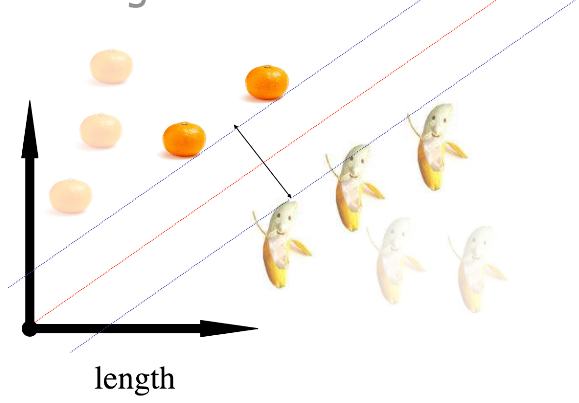
\includegraphics[width=0.5\textwidth]{figures/BananasOranges.png}
    \caption{
      Bananas v Oranges: Margin/Large Deviation Theory}
    \label{Figure 1}
  \end{center}
\end{figure}

\textit{Large Deviation Theory\\}
This idea of maximum margin, where margin is the distance separating bananas from oranges.\\

SVMS are a class of models geared toward finding this margin.

\subsubsection{Example Application - New York Times}

Goal: Want to investigate if there is a link between traffic fatalities and a particular air bag manufacturer - takata\\

To do this, we want to find "interesting cases" so we want to construct some labels/features that classifies a data entry of a particular incident as interesting or not.\\

Example phrases that were interesting were "suddenly deployed" or "unexpectedly". This allowed journalist to find cases and this type of computer assisted reporting led to a massive recall of takata airbags.

\begin{figure}[ht]
  \begin{center}
    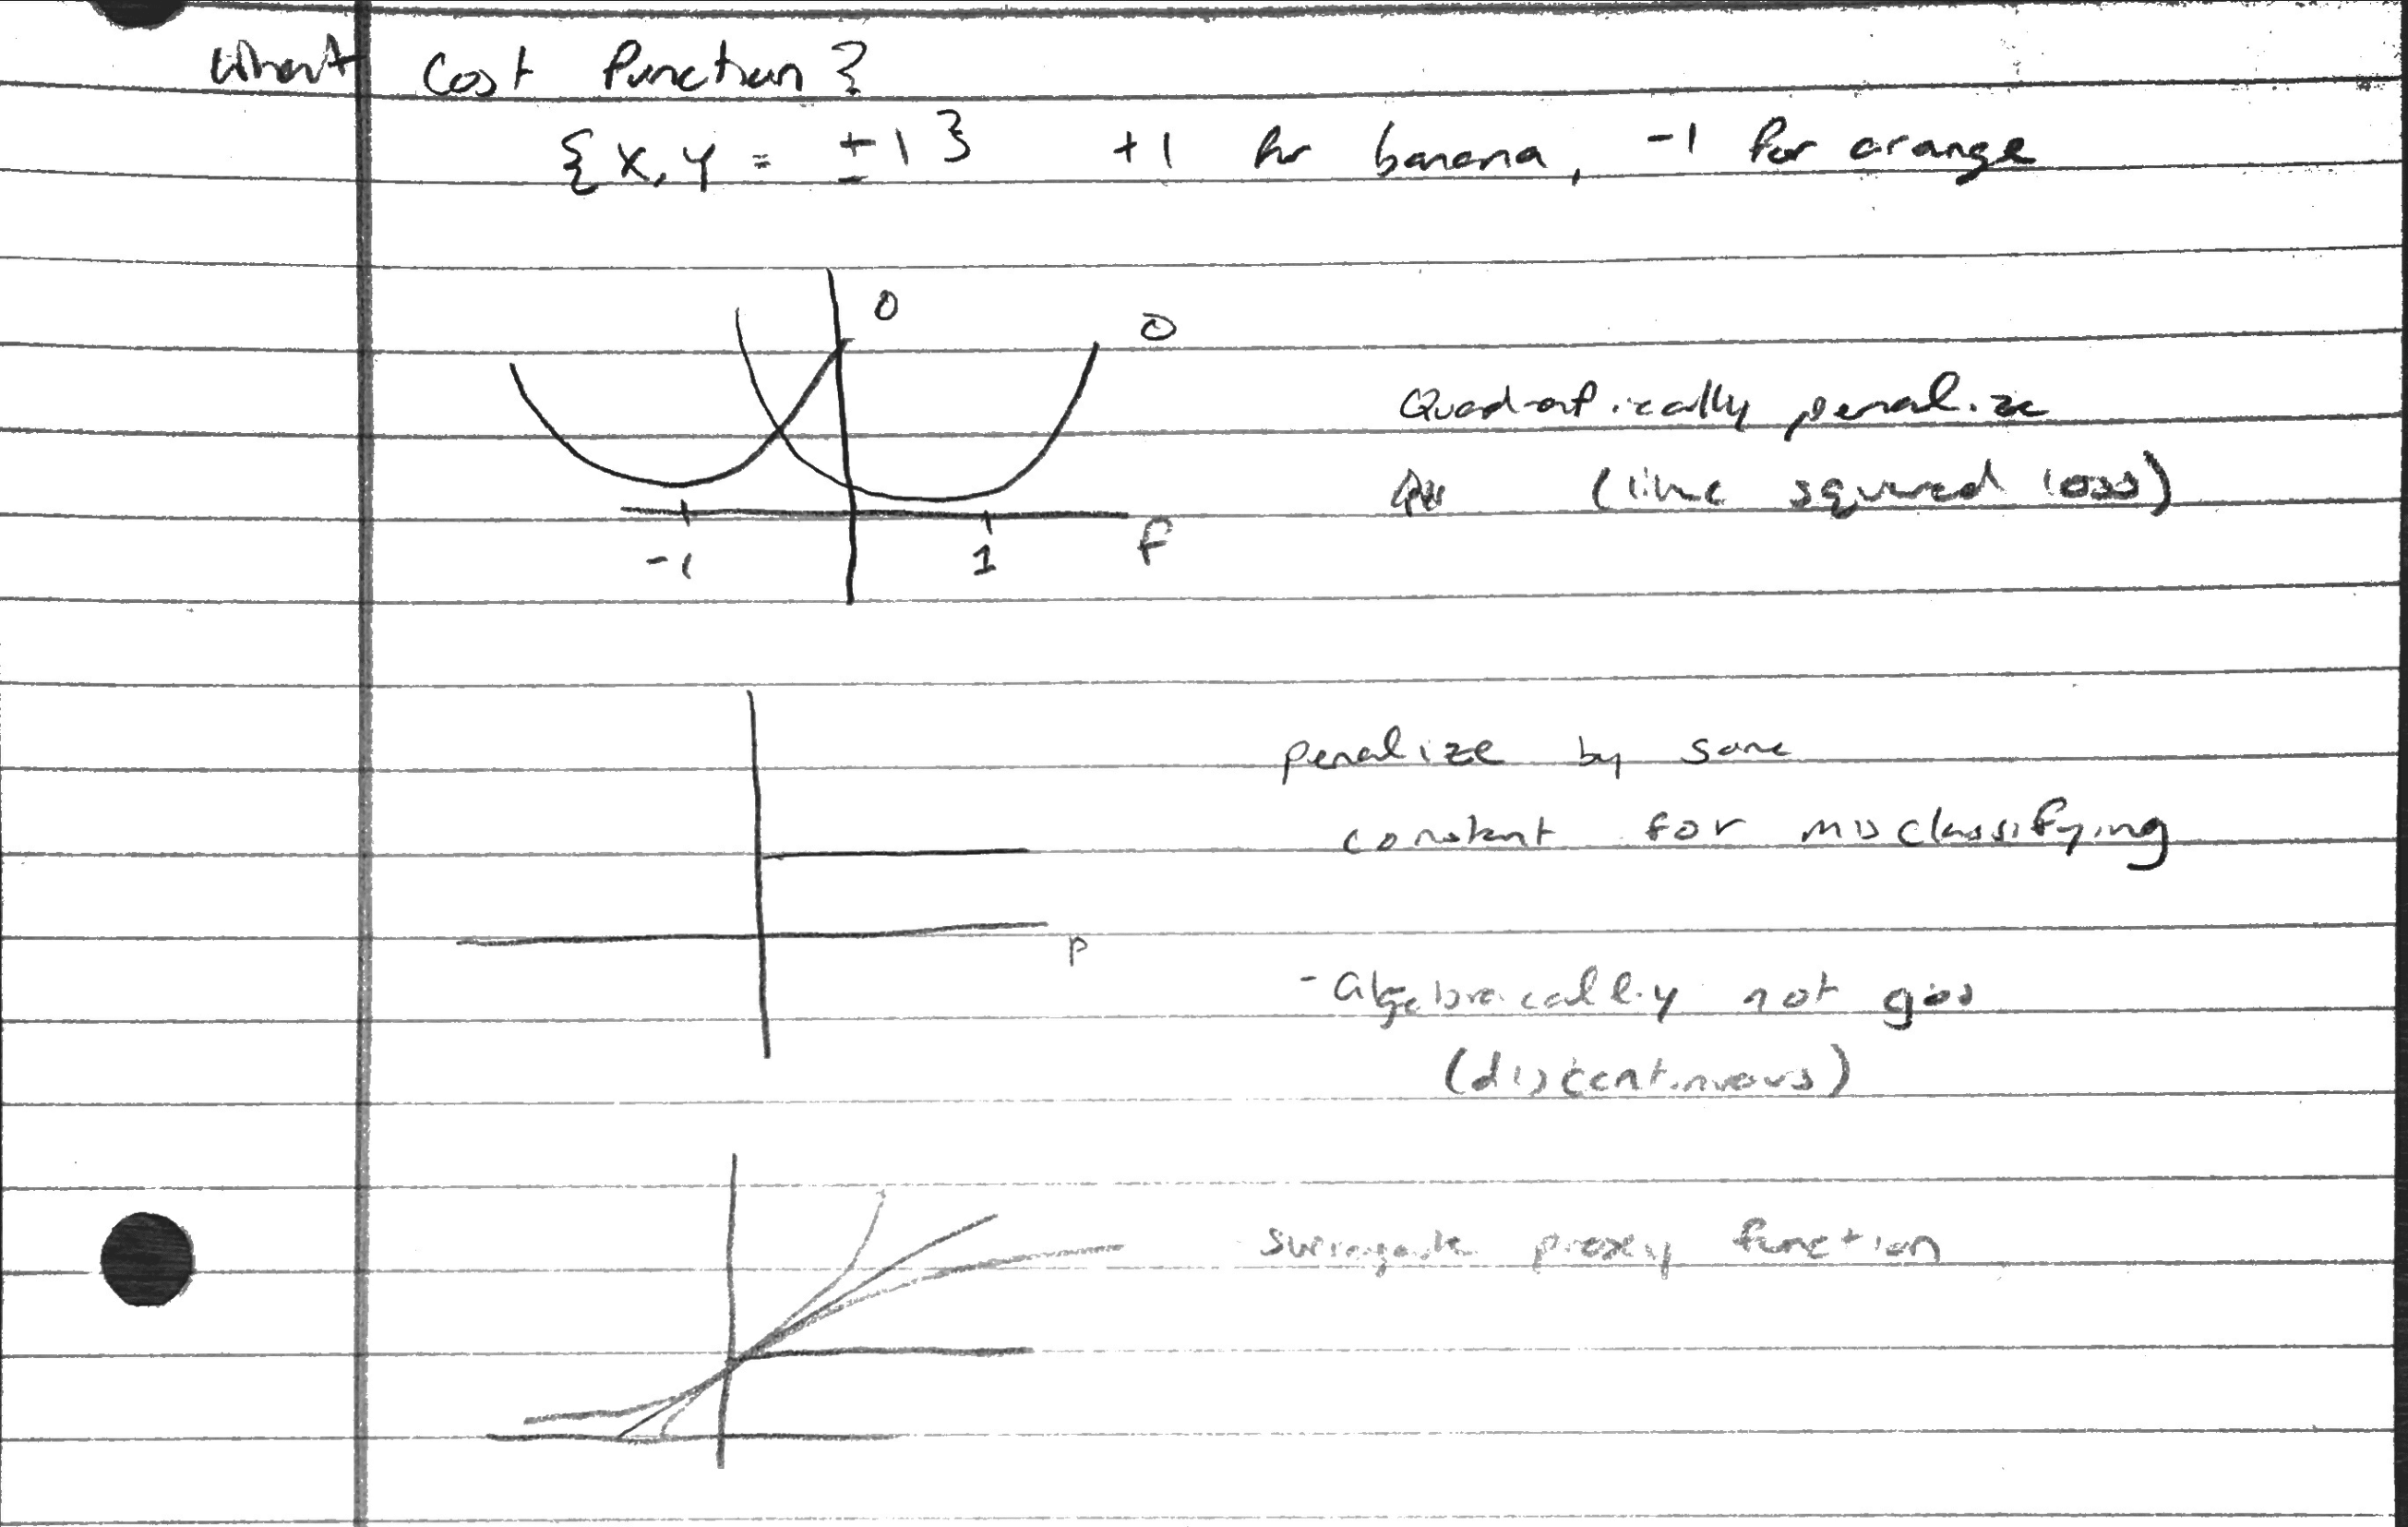
\includegraphics[width=0.5\textwidth]{figures/CostFunctions.png}
    \caption{
      Examples of various cost functions}
    \label{Figure 2}
  \end{center}
\end{figure}

\subsubsection{What is a cost function?}

$${x, y = \pm1} \rightarrow +1 = banana, -1=orange$$

Misclassification often occurs from having no idea on how to step. Support proxy function gives tweaks on how to step. 

\subsubsection{MLE for Classification\\}

Binary/Dichotomous/Boolean features + Naive Bayes\\
Goal: generalize and maintain linearity. Consider the spam problem of recognizing whether a peice of mail is spam.

\paragraph{Example - Bayes Rules Review}
Assume there you are testing for a disease that has infected 1 percent of the population\\

99 percent of sick patients test positive and 99 percent of healthy students test negative. Given that a patient tests positive, what is the probability that the patient is sick?\\

\textit{Bayes Theroem}

$$p(y|x) = \frac{p(x|y)p(y)}{p(x)}$$
$$p(sick|+) = \frac{p(+|sick)p(sick)}{p(+)}$$

$$p(+) = p(+|sick)p(sick)+p(+|healthy)p(healthy)$$

$$p(sick|+) = \frac{p(+|sick)p(sick)}{p(+)} = \frac{99}{198} = 50 \%$$

\paragraph{How does this relate to spam?\\}
Build a one-word spam classifier:

$$p(spam|word) = \frac{p(word|spam)p(spam)}{p(word)}$$

where we just estimate the probabilities as ratios of counts. 

\paragraph{Naive Bayes}
\textit{Naive} comes from the fact that we are assuming every word appears independent of other words.\\

\textit{Bernoulli likelihood}
$$p(x|c) = \prod_j{\theta_{jc}^{x_j} (1-\theta_{jc}^{1-x_{jc}})}$$

Take log-likelihood and derivative to get MLE:

$$log(p(c|x)) = \sum_j{x_j\log{\frac{\theta_{jc}}{1-\theta_{jc}}}+\sum_j{\log{1+\theta_{jc}}}}$$

$$\frac{d}{d\theta}log(p(c|x)) = \frac{\sum_j{x_j}}{\theta}+\frac{\sum_j{1-x_j}}{1-\theta}$$

$$\theta_c = \frac{\sum_j{x_j}}{N}$$

which is just like regression

\subsection{Boosting}

Assume we have a set of training example. We iteratively add weak rules to our model (example: length < 2, etc...). Each feature we add is meant to minimize a loss function which is determined by the weight of our current $x_i$. Weight increases if our new rules gets it right and decreases if the new rule gets it wrong.

\paragraph{Questions on boosting:\\}

What happens if we get a feature with a high weight?

Boosting is extremely resistant to overfitting as we minimize test error.\\

Can a rule become useless?
We can use decision trees or boosted trees. There are different types of boosting methods, each useful for different situations.  

\subsection{Summary}

This lecture gives an introduction to classification showing various methods like naive bayes and boosting. We derived how naive bayes uses MLE and saw how boosting uses this iterative approach of minimizing a loss function and adding weights. We also got a brief introduction to SVMs.
	 
\section{Part II - Code}

\subsection{Revisiting Part I}

How do we deal with discrete and continuous data?\\
With regression, we were able to have and equations like

$$p(y|x) = wx$$

This wont work here since $p(y|x)$ can't take any value between 0 and 1.

$$p(y=1|x) = e^{w_1x}, p(y=0|x) = e^{w_2x}$$

These need to sum to 1 so:

$$p(y=1|x) = \frac{e^{w_1x}}{e^{w_1x}+e^{w_2x}}$$

We can divide through by $e^{w_2x}$ such that

$$p(y=1|x) = \frac{e^{w_3x}}{e^{w_3x}+1}$$

We want to get best w after given some data.\\
\textit{Naive Bayes:} All weight are independent so you can estimate them separately\\
\textit{Boosting} Doesn't assume this so we need to use whole vector

\paragraph{Naive Bayes\\}

Weights are just MLEs so:

$$\log{\frac{p}{1-p}} = wx \rightarrow p(y|x) = \frac{e^{w_3x}}{e^{w_3x}+1}$$

$$w_1x_1+w_2x_2+...$$

Naive Bayes says we can estimate this by just counting. For example, if we are looking at the keyword "money" and whether its spam:

$$\hat{\theta} = \frac{N_{money, spam}}{N_{money}}$$
$$w = \log{\frac{\theta_{money}}{1-\theta_{money}}}$$ 

\subsection{Logistic Regression and Boosting}

\begin{itemize}
	\item Have a cost function for wieght
	\item Do log-likelihood, derivative $\rightarrow$ No closed form sol.
	\item Use principle of iteratively adding weights minimizing cost function (boosting)
\end{itemize}

\subsection{Code}
\subsubsection{Shell Script}

Grab enron dataset which has a bunch of spam and ham email. Use the spam formula from before for Naive Bayes:

$$p(spam|word) = \frac{p(word|spam)p(spam)}{p(word)}$$

Running on "enron" will give 0 which is not good as you are betting enron will never be spam. Thus we can add pseudocounts:

$$p_{money} = \frac{p(money|spam) + \alpha}{p_{spam}+\beta}$$

We can use cross validation to get best a and b.

\subsubsection{R Code}

ELSR dataset for spam. Here we can run naive bayes on training data and create a apriori table. We can then predict on test data and get predicted probabilities for every email. Then we can plot distribution or even bin things and plot a calibration plot.\\

Note: Naive Bayes is over confident since independence of features and multiplying things we are confident about will lead to overconfidence.\\

Logistic regression can correct for overconfidence by considering correlation between things. 


\end{document}

%%% Local Variables:
%%% mode: latex
%%% TeX-master: t
%%% End:
